\subsubsection{Beispiel 1: Der Fluss}

\hfill \break
Berechne die Breite eines Flusses, wenn in einem geradlinigen Uferstück die Standlinie AB (150m) abgesteckt wird
sowie die Winkel CAB (63°22') und CBA (44°30') zu einem am gegenüberliegenden Ufer liegenden Punkt C gemessen
wird.
(Lösung: 98,75m)

\hfill \break
\begin{itemize}
    \item Winkel $CAB = \alpha = 63.37$°
    \item Winkel $CBA = \beta = 44.5$°
    \item Winkel $BC = \gamma = 72.13$°
\end{itemize}

\hfill \break
Rechenweg:\\
\fboxrule=0.8pt \fcolorbox{black}{lightgray}{%
    \begin{tabular}[t]{@{}l@{}}
        $x = \frac{Sin(44.5)*150}{Sin(72.13)}$ \\
        $x = 110.47$                           \\
        \\
        $b=Sin(\alpha)/x$                      \\
        $b=Sin(63.37)*110.47$                  \\
        $b=98.75m$                              \\
    \end{tabular}}

\hfill \break
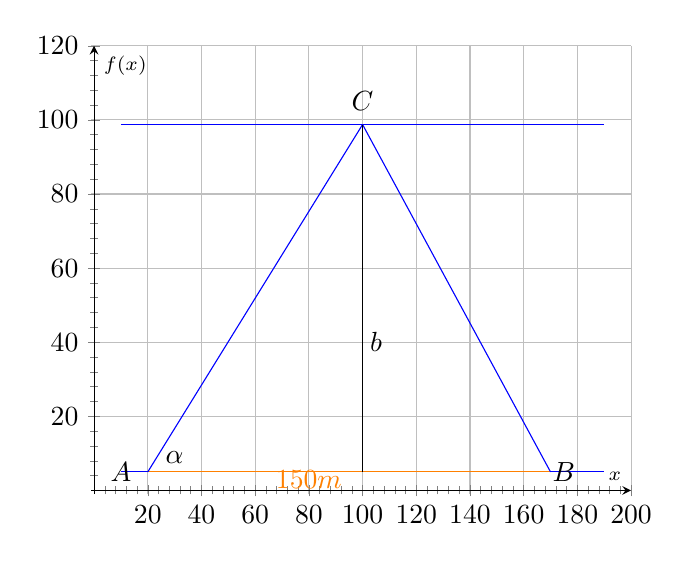
\begin{tikzpicture}[scale=1]
    \begin{axis}%
        [
            grid=major,
            xtick={0,20,...,200},
            minor x tick num=4,
            xmin=-1,
            xmax=200,
            xlabel={\scriptsize $x$},
            axis x line=middle,
            ytick={0,20,...,120},
            minor y tick num=4,
            ymin=-1,
            ymax=120,
            ylabel={\scriptsize $f(x)$},
            axis y line=middle,
            no markers,
            samples=100,
            domain=-1:10,
        ]

        \draw[color=blue] (10,5) -- (190,5);
        \draw[color=orange] (20,5) -- (170,5);
        \draw[color=blue] (10,98.75) -- (190,98.75);
        \draw[color=blue] (100,98.75) -- (20,5);
        \draw[color=blue] (100,98.75) -- (170,5);
        \draw[color=black] (100,98.75) -- (100,5);

        \node[color=black] at (10,5) {$A$};
        \node[color=black] at (175,5) {$B$};
        \node[color=black] at (100,105) {$C$};
        \node[color=black] at (105,40) {$b$};
        \node[color=black] at (30,9) {$\alpha$};
        \node[color=orange] at (80,3) {$150m$};
    \end{axis}
\end{tikzpicture}